\section{Dati e analisi}
Con le impostazioni che ho ricavato nella sezione precedente ho quindi proceduto con la simulazione del comportamento delle onde in presenza di vari potenziali.
\subsection{Potenziali di cui conosco la teoria}
Il primo potenziale che analizzo \`e il salto di potenziale, posiziono un gradino a met\`a del dominio e, con varie altezze e ne calcolo il coefficiente di trasmissivit\`a.

\begin{equation}
\lr\{.{\begin{array}{lr}
	V_0& x>a\\
	0&\text{altrove}
	\end{array}}
\end{equation}

Prima di tutto far\`o una piccola parentesi teorica sul risultato che mi aspetto. Prendiamo un dominio infinito con in 0 il salto di potenziale, l'equazione, indipendente dal tempo, avr\`a la forma:
\begin{equation}
	E\psi = \lrt{-\frac{\hbar^2}{2m}\pde{^2}{x^2}+V_0H(x)}\psi
\end{equation}
Divido lo spazio in due porzioni ($x<0$ e $x>0$) in cui:
\begin{equation}\label{eq:Ks}
	\begin{array}{lr}
	k_1 = \sqrt\frac{2m E}{\hbar}&x<0\\
	k_2 = \sqrt\frac{2m \lrt{E-V_0}}{\hbar}&x>0
	\end{array}
\end{equation}
Dato che il potenziale ha una discontinuit\`a finita in $0$, funzione e derivata devono essere continue. Se per esempio avessimo delle onde piane in ciascuna porzione dello spazio ne avrei una che si muove verso destra ($\psi_\to$) e una verso sinistra ($\psi_\from$) e quindi in 0 avrei, chiamando i coefficenti delle onde piane $A$ per il lato sinistro e $B$ quello destro:
\begin{equation}
	\lr\{.{\begin{array}{lr}
	A_\to e^{ik_1x} + A_\from e^{-ik_1x}	&	x<0\\
	B_\to e^{ik_2x} + B_\from e^{-ik_2x}	&	x>0
	\end{array}}\Rightarrow
	\lr\{.{\begin{array}{l}
	A_\to+A_\from = B_\to+B_\from\\
	k_1\lrt{A_\to-A_\from} = k_2\lrt{B_\to-B_\from}
	\end{array}}
\end{equation}
nel caso pi\`u generico. Nel nostro caso consideriamo un'onda piana da $-\infty$ che si muove verso destra prima di incontrare la barriera:
\begin{equation}
\lr\{.{\begin{array}{ccc}
A_\to = 1&,&
A_\from = r\\
B_\to = t&,&
B_\from=0
\end{array}} \Rightarrow\lr\{.{\begin{array}{l}
	1+r = t\\
	k_1 \lrt{1-r} = k_2 t
\end{array}} \Rightarrow\lr\{.{\begin{array}{l}
	r = \frac{k_1-k_2}{k1+k_2}\\
	t = \frac{2k_1}{k1+k_2}
\end{array}}
\end{equation}
Quelli che mi interessano sono per\`o il coefficiente di riflessione e trasmissione, dato che stiamo parlando di funzioni con norma L2 sono:
\begin{equation}
\lr\{.{\begin{array}{l}
	R = \lr||{r}^2 = \frac{\lrt{k_1-k_2}^2}{\lrt{k1+k_2}^2}\\
	T = 1-R = \lr||{t}^2\frac{k_2}{k_1} = \frac{4 k_1 k_2}{\lrt{k1+k_2}^2}
\end{array}}
\end{equation}

\begin{figure}[hbt]
	\centering
	\begin{tikzpicture}
	\begin{axis}[axis x line = center, axis y line = center, xlabel=E/V, xlabel style={below}, xmin = -0.1, xmax = 3.1, ymin=-0.1,ymax =1.1]
		\addplot[domain=0:3, samples =501, red]		plot[id=Trasm]	function{x<1?0:1-(-1+sqrt(1-1/x))*(-1+sqrt(1-1/x))/((1+sqrt(1-1/x))*(1+sqrt(1-1/x)))};
		\addplot[domain=0:3, samples =501, blue]	plot[id=Refl]	function{x<1?1:(-1+sqrt(1-1/x))*(-1+sqrt(1-1/x))/((1+sqrt(1-1/x))*(1+sqrt(1-1/x)))};
	\end{axis}
	\end{tikzpicture}
	\caption{Coefficienti di trasmissione in rosso e riflessione in blu}
\end{figure}

Quindi proseguiamo ed eseguiamo delle simulazioni.

Nelle simulazioni i lanci sono stati fatti con pacchetti gaussiani inizialmente con $\sigma=0.5$, energia $100$ e massa $10$. Il potenziale \`e stato impostato perch\'e il salto fosse al centro del dominio e con altezza diversa per ogni lancio: $10,\ 25,\ 50,\ 75,\ 100,\ 200,\ 300$ e ne ho analizzato l'andamento temporale del rapporto tra l'integrale su tutto il dominio e quello fatto nella prima met\`a, ricavando cos\`i il coefficiente di riflessione nel tempo. Il coefficiente di riflessione possiamo dire che \`e il valore del peso dell'integrale quando si \`e stabilizzato dall'andamento nel tempo si pu\`o vedere un piccolo abbassamento quando l'onda impatta il potenziale, prima di venire riflessa all'indietro penetra leggermente nell'area classicamente vietata.

\begin{figure}[tbh]
\centering
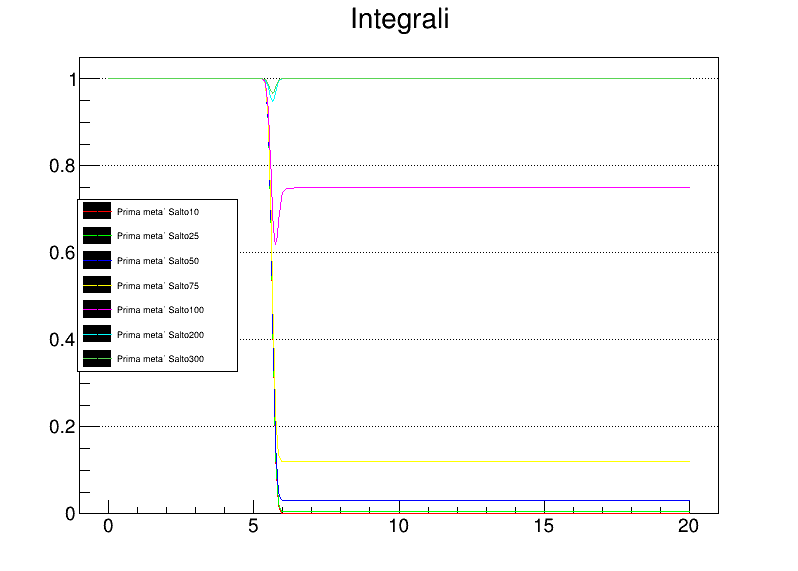
\includegraphics[width=0.7\linewidth]{IMG/SaltoR}
\caption{I pesi dell'integrale della prima met\`a del dominio per $\sigma=0.5$}\label{fig:SaltoR}
\end{figure}

Come si pu\`o notare dalla \autoref{tab:SaltoDati} sebbene stia simulando un pacchetto d'onda in movimento e non un un'onda piana il peso dei coefficienti ricalca abbastanza bene i coefficienti teorici, e sembra avvicinarli di pi\`u man mano che allargo il pacchetto. Notare che la simulazione si allontana dalla teoria per le onde piane man mano che mi avvicini al regime in cui il potenziale \`e maggiore dell'energia dell'onda.

\begin{table}[hbt]
	\centering
\begin{tabular}{cccccc}
\toprule
\multirow{2}{*}{E/V}&\multicolumn{4}{c}{simulazione $\sigma$}		& \multirow{2}{*}{teoria}		\\ \cmidrule(lr){2-5}
					&$0.5$			&$1$			&$2$			&$4$			&				\\ \midrule
$10$				&$0.000724389$	&$0.000718394$	&$0.000716913$	&$0.000716543$	&$0.000693482$	\\ \midrule
$4$					&$0.00539149$	&$0.00533663$	&$0.00532312$	&$0.00531976$	&$0.00515478$	\\ \midrule
$2$					&$0.0309848$	&$0.0304801$	&$0.0303576$	&$0.0303272$	&$0.0294373$	\\ \midrule
$1.66$				&$0.0536892$	&$0.0525454$	&$0.0522718$	&$0.0522041$	&$0.0506914$	\\ \midrule
$1.33$				&$0.120552$		&$0.1158$		&$0.114741$		&$0.114483$		&$0.111112$		\\ \midrule
$1.11$				&$0.344071$		&$0.291725$		&$0.281975$		&$0.279959$		&$0.269876$		\\ \midrule
$1$					&$0.751078$		&$0.815668$		&$0.8777$		&$0.934287$		&$1$			\\ \midrule
$0.9090$			&$0.978315$		&$0.999843$		&$1$			&$1$			&$1$			\\ \midrule
$0.8$				&$0.999979$		&$1$			&$1$			&$1$			&$1$			\\ \midrule
$0.5$				&$1$			&$1$			&$1$			&$1$			&$1$			\\ \midrule
$0.33$				&$1$			&$1$			&$1$			&$1$			&$1$			\\ \bottomrule
\end{tabular}
\caption{Alcuni dati delle simulazioni per il salto di potenziale}\label{tab:SaltoDati}
\end{table}

\begin{figure}[hbt]
	\centering
	\begin{tikzpicture}
	\begin{axis}[axis x line = center, axis y line = center, xlabel=E/V, xlabel style={below right}, xmin = -0.1, xmax = 10.1, ymin=-0.1,ymax =1.1]
	\addplot table[x=ev,y=fhS1] {Dati/pesi2.dat};%{Dati/Salto.dat};
	\addlegendentry{$\sigma=0.5$}
	\addplot table[x=ev,y=fhS2] {Dati/pesi2.dat};
	\addlegendentry{$\sigma=1$}
	\addplot table[x=ev,y=fhS3] {Dati/pesi2.dat};
	\addlegendentry{$\sigma=2$}
	\addplot table[x=ev,y=fhS4] {Dati/pesi2.dat};
	\addlegendentry{$\sigma=4$}
	\addplot[domain=0:10, samples =501, blue]	plot[id=Refl2]	function{x<1?1:(-1+sqrt(1-1/x))*(-1+sqrt(1-1/x))/((1+sqrt(1-1/x))*(1+sqrt(1-1/x)))};
	\addlegendentry{teoria}
	\end{axis}
	\end{tikzpicture}
	\caption{La visualizzazione dei dati e il confronto con la teoria}
\end{figure}

\subsection{La barriera}
Similmente a prima usiamo le definizioni dei $k$ in \eqref{eq:Ks}. Il potenziale avr\`a la forma:

\begin{equation}
\lr\{.{\begin{array}{lr}
	V_0& 0<x<a\\
	0&\text{altrove}
	\end{array}}
\end{equation}
Per l'esempio $x_0=0$.

Dato che il potenziale ha una discontinuit\`a finita in $a$ e in $-a$, funzione e derivata devono essere continue. C0me prima:
\begin{equation}
	\lr\{.{\begin{array}{lr}
		A_\to e^{ik_1x} + A_\from e^{-ik_1x}	&	x<0\\
		C_\to e^{ik_2x} + C_\from e^{-ik_2x}	&	0<x<a\\
		B_\to e^{ik_1x} + B_\from e^{-ik_1x}	&	x>a
	\end{array}}\Rightarrow\lr\{.{\begin{array}{lr}
		A_\to  +A_\from = C_\to+C_\from															&	\text{in }0\\
		C_\to e^{ik_2a}+C_\from e^{-ik_2a} = B_\to e^{ik_1a} +B_\from e^{-ik_1a}				&	\text{in }a\\
		k_1\lrt{A_\to e^{-ik_1a}-A_\from e^{ik_1a}}=k_2\lrt{C_\to e^{-ik_2a}-C_\from e^{ik_2a}}	&	\text{in }0\\
		k_2\lrt{C_\to e^{ik_2a}-C_\from e^{-ik_2a}}=k_1\lrt{B_\to e^{ik_1a}-B_\from e^{-ik_1a}}	&	\text{in }a
	\end{array}}
\end{equation}
nel caso pi\`u generico. Nel nostro caso consideriamo un'onda piana da $-\infty$ che si muove verso destra prima di incontrare la barriera:
\begin{equation}
\lr\{.{\begin{array}{ccc}
	A_\to = 1&,&
	A_\from = r\\
	B_\to = t&,&
	B_\from=0\\
	C_\to = m_1&,&
	C_\from=m_2
	\end{array}} \Rightarrow\lr\{.{\begin{array}{l}
	1+r= m_1 +m_2 \\
	m_1 e^{ik_2a}+m_2 e^{-ik_2a} = t e^{ik_1a}\\
	k_1\lrt{1 - r}=k_2\lrt{m_1 - m_2}\\
	k_2\lrt{m_1 e^{ik_2a}-m_2 e^{-ik_2a}}=k_1 t e^{ik_1a}
	\end{array}} \Rightarrow\lr\{.{\begin{array}{l}
	r = -\frac{4 e^{-i a \lrt{k_1-k2}} k_1 k_2}{\lrt{k_1-k_2}^2 e^{2 i a k_2}-\lrt{k_1+k_2}^2}\\
	t = \frac{\lrt{e^{2 i a k_2}-1}\lrt{k_1^2-k_2^2}}{\lrt{k_1-k_2}^2 e^{2 i a k_2}-\lrt{k_1+k_2}^2}\\
	m_1 = -\frac{2k_1\lrt{k_1+k_2}}{\lrt{k_1-k_2}^2 e^{2 i a k_2}-\lrt{k_1+k_2}^2}\\
	m_2 = \frac{2 e^{2 i a k_2}k_1\lrt{k_2-k_1}}{\lrt{k_1-k_2}^2 e^{2 i a k_2}-\lrt{k_1+k_2}^2}
	\end{array}}
\end{equation}

ma  a noi interessano:

\begin{equation}
\lr\{.{\begin{array}{l}
	R = \lr||{r}^2 = \lr||{\frac{2e^{-i a k_1}k_1 k_2}{i\lrt{k_1+k_2}^2 \sin\lrt{a k_2}-2k_1 k_2 \cos\lrt{a k_2}}}^2=
	\frac{4 k_1^2 k_2^2}{4 k_1^2 k_2^2 \cos^2\lrt{a k_2}+\lrt{k_1^2+k_2^2}^2\sin^2\lrt{(a k_2)}}\\
	T = \lr||{t}^2 = \lr||{\frac{\sin\lrt{a k_2}\lrt{k_1^2-k_2^2}}{\lrt{k_1+k_2}^2 \sin\lrt{a k_2}+2 i k_1 k_2 \cos\lrt{a k_2}}}^2=
	\frac{\lrt{k_1^2-k_2^2}^2\sin^2\lrt{(a k_2)}}{4 k_1^2 k_2^2 \cos^2\lrt{a k_2}+\lrt{k_1^2+k_2^2}^2\sin^2\lrt{(a k_2)}}
	\end{array}}
\end{equation}

\begin{figure}[hbt]
	\centering
	\begin{tikzpicture}
	\begin{axis}[axis x line = center, axis y line = center, xlabel=E/V, xlabel style={below right}, xmin = -0.1, xmax = 10.1, ymin=-0.1,ymax =1.1]
	\addplot table[x=ev,y=L2] {Dati/pesiMurog1.dat};%{Dati/Salto.dat};
	\addlegendentry{$2$}
%	\addplot table[x=ev,y=L4] {Dati/pesiMurog1.dat};
%	\addlegendentry{$4$}
	\addplot table[x=ev,y=L2] {Dati/pesiMurog2.dat};
	\addlegendentry{$2$}
	\addplot table[x=ev,y=L2] {Dati/pesiMurog3.dat};
	\addlegendentry{$2$}
	\addplot table[x=ev,y=L2] {Dati/pesiMurog4.dat};
	\addlegendentry{$2$}
%	\addplot table[x=ev,y=L2] {Dati/pesiMurog2.dat};
%	\addlegendentry{$4$}
%	\addplot table[x=ev,y=L16] {Dati/pesiM.dat};
%	\addlegendentry{$16$}
%(2*sin(20*a*sqrt(5 - 5/x))*sin(20*a*sqrt(5 - 5/x)))/(1 - 8*x + 8*x*x - cos(40*a*sqrt(5 - 5/x)))
	\addplot[domain=1.00000001:10, samples =501, blue]	plot[id=MRefl2]	function{(2*sin(20*2*sqrt(5 - 5/x))*sin(20*2*sqrt(5 - 5/x)))/(1 - 8*x + 8*x*x - cos(40*2*sqrt(5 - 5/x)))};
	\addlegendentry{teoria 2 }
%	\addplot[domain=1.00000001:10, samples =501, green]	plot[id=MRefl2]	function{(2*sin(20*4*sqrt(5 - 5/x))*sin(20*4*sqrt(5 - 5/x)))/(1 - 8*x + 8*x*x - cos(40*4*sqrt(5 - 5/x)))};
%	\addlegendentry{teoria 4 }
%	\addplot[domain=0:10, samples =501, red]	plot[id=MRefl2]	function{(-2*sin(4*sqrt(-1 + x))*sin(4*sqrt(-1 + x)))/(-1 + 8*x - 8*x*x + cos(2*4*sqrt(-1 + x)))};
%	\addlegendentry{teoria 4}
%	\addplot[domain=0:10, samples =501, green]	plot[id=MRefl2]	function{(-2*sin(8*sqrt(-1 + x))*sin(8*sqrt(-1 + x)))/(-1 + 8*x - 8*x*x + cos(2*8*sqrt(-1 + x)))};
%	\addlegendentry{teoria 8}
	\end{axis}
	\end{tikzpicture}
	\caption{La visualizzazione dei dati e il confronto con la teoria}
\end{figure}

\begin{figure}[hbt]
	\centering
	\begin{tikzpicture}
	\begin{axis}[axis x line = center, axis y line = center, xlabel=E/V, xlabel style={below right}, xmin = 1.9, xmax = 4.1, ymin=-0.1,ymax =0.2]
	\addplot table[x=ev,y=L2] {Dati/pesiOscg1.dat};%{Dati/Salto.dat};
	\addlegendentry{$2$}
	\addplot table[x=ev,y=L2] {Dati/pesiOscg2.dat};
	\addlegendentry{$2$}
%	\addplot table[x=ev,y=L2] {Dati/pesiOscg3.dat};
%	\addlegendentry{$2$}
%	\addplot table[x=ev,y=L2] {Dati/pesiOscg4.dat};
%	\addlegendentry{$2$}
	\addplot[domain=2:4, samples =501, blue]	plot[id=MRefl2z]	function{(2*sin(20*2*sqrt(5 - 5/x))*sin(20*2*sqrt(5 - 5/x)))/(1 - 8*x + 8*x*x - cos(40*2*sqrt(5 - 5/x)))};
	\addlegendentry{teoria 2 }
	%	\addplot[domain=1.00000001:10, samples =501, green]	plot[id=MRefl2]	function{(2*sin(20*4*sqrt(5 - 5/x))*sin(20*4*sqrt(5 - 5/x)))/(1 - 8*x + 8*x*x - cos(40*4*sqrt(5 - 5/x)))};
	%	\addlegendentry{teoria 4 }
	%	\addplot[domain=0:10, samples =501, red]	plot[id=MRefl2]	function{(-2*sin(4*sqrt(-1 + x))*sin(4*sqrt(-1 + x)))/(-1 + 8*x - 8*x*x + cos(2*4*sqrt(-1 + x)))};
	%	\addlegendentry{teoria 4}
	%	\addplot[domain=0:10, samples =501, green]	plot[id=MRefl2]	function{(-2*sin(8*sqrt(-1 + x))*sin(8*sqrt(-1 + x)))/(-1 + 8*x - 8*x*x + cos(2*8*sqrt(-1 + x)))};
	%	\addlegendentry{teoria 8}
	\end{axis}
	\end{tikzpicture}
	\caption{I dati tra 2 e 4}
\end{figure}